\documentclass[letterpaper,11pt]{article}

% Soporte para los acentos.
\usepackage[utf8]{inputenc}
\usepackage[T1]{fontenc}
% Idioma español.
\usepackage[spanish,mexico, es-tabla]{babel}
% Soporte de símbolos adicionales (matemáticas)
\usepackage{multirow}
\usepackage{amsmath}
\usepackage{amssymb}
\usepackage{amsthm}
\usepackage{amsfonts}
\usepackage{mathtools}
\usepackage{latexsym}
\usepackage{enumerate}
\usepackage{listings}
\usepackage[dvipsnames]{xcolor}
\usepackage{float}
\usepackage{graphicx}
\usepackage[linguistics]{forest}

% Modificamos los márgenes del documento.                                       
\usepackage[lmargin=1.5cm,rmargin=1.5cm,top=1.5cm,bottom=1.5cm]{geometry}

\title{Facultad de Ciencias, UNAM \\ 
       Análisis de Algoritmos \\ 
       Tarea 3}
\author{Rubí Rojas Tania Michelle}
\date{11 de diciembre de 2020}

\begin{document}
\maketitle

\begin{enumerate}
    % Ejercicio 1.
    \item Un pescador está sobre un océano rectangular. El valor del pez en el 
    punto $(i, j)$ está dado por un arreglo $A$ de dimensión $2 (n \times m)$.
    Diseña un algoritmo que calcule el máximo valor de pescados que un pescador
    puede atrapar en un camino desde la esquina superior izquierda a la esquina 
    inferior derecha. El pescador sólo puede moverse hacia abajo o hacia la 
    derecha, como se ilustra en la siguiente figura: 
    \begin{figure}[h]
        \centering
        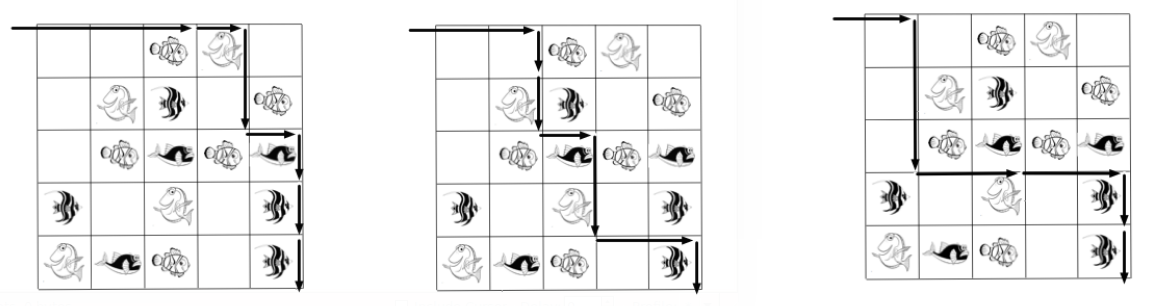
\includegraphics[width=0.5\linewidth]{imagenes/ejercicio1.png}
    \end{figure}

    \textsc{Solución:} Queremos encontrar el máximo valor de peces que podemos 
    obtener al realizar únicamente movimiéntos hacia la derecha y hacia abajo. 
    Así, nuestro objetivo será modificar la matriz $A$ de tal manera que en 
    cada sub-instancia del problema tengamos en $A[i][j]$ el valor máximo de 
    pescaditos que el pescador puede atrapar desde $A[0][0]$ hasta $A[i][j]$
    realizando sólo dos tipos de movimiéntos. De esta forma, al tener cada 
    celda de $A$ actualizada como describimos anteriormente, al final bastará 
    regresar el valor de $A[n-1][m-1]$, pues ésta contendrá el valor máximo 
    de pescaditos que deseamos. 

    Así, consideremos los siguientes puntos:
    \begin{itemize}
        \item El caso base sería que la celda $A[0][0]$ no puede ser 
        actualizada. Esto se debe a que el valor en esa celda es el máximo 
        que el pescador puede obtener si va desde $A[0][0]$ a $A[0][0]$ (no 
        se mueve).

        \item Para el primer renglón de $A$, bastará con ir obteniéndo la 
        suma acumulada de la celda inmediatamente a la izquierda de la 
        actual. Si pensamos que el pescador se está moviéndo siempre hacia 
        la derecha en la primer fila, es decir, el pescador sólo se mueve 
        sobre $A[0][j]$ con $j \in \{0, \ldots, m-1\}$; entonces 
        \begin{equation*}
            A[0][j] = A[0][j-1] + A[0][j]
        \end{equation*}

        Esto se debe a que al sumar el valor de la celda actual que tiene el 
        valor del pez en ese lugar, junto con el máximo que puede obtener el 
        pescador moviéndose solamente hacia la derecha desde $M[0][0]$ hasta 
        una celda previa que ya contiene el máximo, entonces obtenemos el 
        valor deseado. 

        \begin{proof}
            Inducción sobre la columna $j$.
            \begin{itemize}
                \item \textcolor{blue}{Caso base.} Cuando $j = 0$, entonces 
                $A[0][0]$ tiene ya el máximo valor que el pescador puede 
                obtener (por el punto anterior).

                \item \textcolor{blue}{Hipótesis de inducción.} Supongamos que 
                se cumple para $k$, es decir, supongamos que $A[0][k]$ tiene el 
                valor máximo que el pescador puede obtener moviéndose siempre a 
                la derecha sobre el primer renglón hasta ese punto.  

                \item \textcolor{blue}{Paso inductivo.} Queremos probar que se 
                cumple para $A[0][k+1]$. Entonces 
                \begin{align*}
                    A[0][k+1]
                     &= A[0][k] + A[0][k+1] 
                     && \text{por definición}
                \end{align*}

                Por hipótesis de inducción tenemos que $A[0][k]$ tiene el 
                valor máximo que el pescador puede obtener moviéndose a la 
                derecha desde $A[0][0]$ hasta $A[0][k]$. Así, para obtener el 
                máximo hasta la celda que le sigue a la derecha, basta con 
                sumarle el valor que tiene actualmente. Por lo tanto, si 
                actualizamos $A[0][k+1]$ con $A[0][k] + A[0][k+1]$ entonces 
                obtendremos el valor máximo hasta este punto.
            \end{itemize}

            Por lo tanto, si hacemos que $A[0][j] = A[0][j-1] + A[0][j]$, 
            entonces obtendremos en cada celda del primer renglón el valor 
            máximo que el pescador puede conseguir moviéndose siempre a la 
            derecha sobre el primer renglón. 

        \end{proof}

        \item De manera análoga, tenemos el caso para la primer columna 
        de $A$. Será suficiente con ir obteniéndo la suma acumulada de la 
        celda inmediatamente arriba de la actual. Si pensamos que el 
        pescador siempre se está moviéndo hacia abajo en la primer columna, 
        es decir, el pescador sólo se mueve sobre $A[i][0]$ con 
        $i \in \{0, 1, \ldots, n-1\}$; entonces 
        \begin{equation*}
            A[i][0] = A[i-1][0] + A[i][0]
        \end{equation*}

        Esto se debe a que al sumar el valor de la celda actual que tiene 
        el valor del pez en ese lugar, junto con el máximo que puede obtener 
        el pescador moviéndose solamente hacia abajo desde $A[0][0]$ hasta 
        una celda previa que ya contiene el máximo, entonces obtenemos el 
        valor deseado. 
        \begin{proof}
            Inducción sobre el renglón $i$.
            \begin{itemize}
                \item \textcolor{blue}{Caso base}. Cuando $i = 0$, entonces 
                $A[0][0]$ tiene ya el máximo valor que el pescador puede 
                obtener (por el primer punto).

                \item \textcolor{blue}{Hipótesis de inducción}. Supongamos que 
                se cumple para $k$, es decir, supongamos que se cumple que 
                $A[k][0]$ tiene el valor máximo que el pescador puede obtener 
                moviéndose siempre hacia abajo sobre la primer columna hasta 
                ese punto.  

                \item \textcolor{blue}{Paso inductivo}. Queremos probar que se 
                cumple para $A[k+1][0]$. Entonces 
                \begin{align*}
                    A[k+1][0] &= A[k][0] + A[k+1][0]
                    && \text{por definición} 
                \end{align*}

                Por hipótesis de inducción tenemos que $A[k][0]$ tiene el valor 
                máximo que el pescador puede obtener moviéndose a la derecha 
                desde $A[0][0]$ hasta $A[k][0]$. Así, para obtener el máximo 
                hasta la celda que le sigue abajo, basta con sumarle el valor 
                que tiene actualmente. Por lo tanto, si actualizamos 
                $A[k+1][0]$ con $A[k][0] + A[k+1][0]$, entonces obtendremos el 
                valor máximo hasta este punto. 
            \end{itemize}

            Por lo tanto, si hacemos que $A[i][0] = A[i-1][0] + A[i][0]$, 
            entonces obtendremos en cada celda de la primer columna el valor 
            máximo que el pescador puede conseguir moviéndose siempre hacia 
            abajo sobre la primer columna.

        \end{proof}

        \item Para actualizar la parte de la matriz $A$ que falta, entonces 
        es suficiente considerar el valor actual de cada celda que contiene
        el valor del pez en ese lugar del océano junto con el máximo valor 
        en las celdas inmediatamente arriba y a la izquierda de la actual, 
        es decir, 
        \begin{equation*}
            A[i][j] = A[i][j] + max\left\{A[i-1][j], A[i][j-1] \right\}
        \end{equation*}

        Esto lo haremos para las entradas $(i,j)$ con  
        $i \in \{1, \ldots, n-1\}, j \in \{1, \ldots, j-1\}$.

        Mostraremos que gracias a esta expresión, cada celda tendrá el 
        valor máximo que el pescador puede conseguir moviéndose desde 
        $M[0][0]$ hasta $M[i][j]$ con movimiéntos únicamente hacia la 
        derecha o hacia abajo.
        \begin{proof}
            Inducción sobre el renglón $i$.
            \begin{itemize}
                \item \textcolor{blue}{Caso base}. Como $i=1$, entonces 
                debemos mostrar que
                \begin{equation*}
                    A[1][j] = 
                    A[1][j] + max\left\{A[0][j], A[1][j-1] \right\}
                \end{equation*}

                \begin{proof}
                    Inducción sobre la columna $j$.
                    \begin{itemize}
                        \item \textcolor{purple}{Caso base}. Como $j=1$, 
                        entonces
                        \begin{equation*}
                            A[1][1] = 
                            A[1][1] + max\left\{A[0][1], A[1][0] \right\}
                        \end{equation*} 

                        Así, tendremos que $A[1][1]$ contiene el máximo valor 
                        que el pescador puede conseguir moviéndose solamente 
                        a la derecha o hacia abajo desde $A[0][0]$ y hasta 
                        $A[1][1]$. Por las demostraciones anteriores sabemos
                        que $A[0][1]$ ya tiene el máximo valor que puede 
                        conseguir el pescador moviéndose solamente hacia la 
                        derecha de la posición inicial y $A[1][0]$ ya tiene 
                        el máximo valor que puede conseguir el pescador 
                        moviéndose solamente hacia abajo desde $A[0][0]$. 
                        Entonces basta con sumarle el valor de la celda actual 
                        $A[1][1]$ al valor más grande de las dos opciones 
                        que se tienen por la restricción de los movimientos 
                        para obtener el valor máximo deseado. Por lo tanto, 
                        este caso se cumple. 

                        \item \textcolor{purple}{Hipótesis de inducción}. 
                        Supongamos que se cumple para $k$, es decir, supongamos
                        que $A[1][k]$ tiene el valor máximo que el pescador 
                        puede obtener moviéndose con las restricciones dadas
                        hasta ese punto desde $A[0][0]$.

                        \item \textcolor{purple}{Paso inductivo}. Queremos 
                        probar que se cumple para $A[1][k+1]$. Entonces 
                        \begin{align*}
                            A[1][k+1] 
                            &= A[1][k+1] + max\left\{A[0][k+1], A[1][k] \right\}
                            && \text{por definición}
                        \end{align*}

                        Por el paso inductivo del primer renglón tenemos que 
                        $A[0][k+1]$ ya tiene el máximo valor que puede obtener el 
                        pescador moviéndose solamente hacia la derecha. Luego, 
                        por hipótesis de inducción, $A[1][k]$ ya tiene el máximo
                        valor que el pescador puede obtener moviéndose con las 
                        restricciones dadas hasta ese punto desde $A[0][0]$. Así, 
                        al considerar el valor máximo de estos dos óptimos, se 
                        obtiene el óptimo al moverse a la derecha o hacia abajo 
                        desde $A[0][0]$; y solo falta sumar el valor actual de 
                        $A[1][k+1]$ para obtener el máximo valor deseado. 
                    \end{itemize}
                \end{proof}

                \item \textcolor{blue}{Hipótesis de inducción}. Supongamos que 
                se cumple para $k$, es decir, supongamos que $A[k][j]$ tiene 
                el valor máximo que el pescador puede obtener moviéndose hacia 
                abajo o hacia la derecha desde $A[0][0]$ hasta $A[k][j]$. 

                \item \textcolor{blue}{Paso inductivo}. Queremos mostrar que se 
                cumple para $k+1$. Entonces 
                \begin{align*}
                    A[k+1][j] 
                    &= A[k+1][j] + max\left\{A[k][j], A[k][j-1] \right\}
                \end{align*}

                Por hipótesis de inducción tenemos que $A[k][j], A[k][j-1]$ 
                tienen ya el valor máximo que el pescador puede obtener 
                moviéndose hacia abajo o hacia la derecha desde $A[0][0]$
                hasta $A[k][j]$ y $A[k][j-1]$, respectivamente. Así, al 
                considerar el valor máximo de estos dos, se obtiene el 
                óptimo deseado. Así, sumando el valor actual de $A[k+1][j]$
                obtenemos el valor máximo buscado. 
            \end{itemize}

            Por lo tanto, cada entrada $(i,j)$ de la matriz $A$ con 
            $i \in \{1, \ldots, n-1\}$ y $j \in \{1, \ldots, m-1\}$ tendrá 
            el valor máximo que el pescador puede obtener moviéndose solamente 
            a la derecha o hacia abajo desde el punto inicial $A[0][0]$ si 
            \begin{equation*}
                A[i][j] = A[i][j] + max\left\{A[i-1][j], A[i][j-1] \right\}
            \end{equation*}
        \end{proof}
    \end{itemize}

    \newpage
    Esto lo podemos traducir como el siguiente algoritmo:
    \begin{itemize}
        \item[1.] Definimos $i = j = 0$.

        \item[2.] Mientras $j$ sea menor que $m$, hacemos
        \begin{equation*}
            A[0][j] = A[0][j-1] + A[0][j]
        \end{equation*}

        Aumentamos en una unidad a $j$.

        \item[3.] Mientras $i$ sea menor que $n$, hacemos 
        \begin{equation*}
            A[i][0] = A[i-1][0] + A[i][0]
        \end{equation*}

        Aumentamos en una unidad a $i$.

        \item[4.] Definimos $i = j = 1$.

        \item[5.] Mientras $i$ sea menor que $n$, hacemos 
        \begin{itemize}
            \item Mientras $j$ sea menor que $m$, hacemos 
            \begin{equation*}
                A[i][j] = A[i][j] + max\left\{A[i-1][j], A[i][j-1]\right\}
            \end{equation*}

            Aumentamos en una unidad a $j$.
        \end{itemize}

        Aumentamos en una unidad a $i$.

        \item[6.] Regresamos $A[n-1][m-1]$.
    \end{itemize}

    Ahora bien, los ciclos \texttt{while} de los pasos $2$ y $3$ nos toman 
    $\Theta(m)$ y $\Theta(n)$, respectivamente; pues estamos recorriendo una 
    sola vez un renglón y una columna. Y el ciclo \texttt{while} del paso $5$
    nos toma $\Theta(nm)$, ya que estamos recorriendo lo que queda de la 
    matriz $A$ (entrada por entrada). Por lo tanto, la complejidad total del 
    algoritmo es de $\Theta(nm)$.

    % Ejercicio 2.
    \item Dados dos árboles generadores $T$ y $R$ de una gráfica $G$. Muestra 
    cómo encontrar la secuencia más corta de árboles generadores $T_0, T_1, 
    \ldots, T_k$ tal que $T_0 = T, T_k = R$, y cada árbol $T_i$ difiere del 
    anterior $T_{i-1}$ agregando y borrando una arista.

    % Ejercicio 3.
    \item Sea $G$ una gráfica con $n$ vértices. Un subconjunto $S$ de los 
    vértices de $G$ es independiente si cualesquiera dos elementos de $S$ no 
    son adyacentes. En general, el problema de encontrar el conjunto 
    independiente de una gráfica es un problema $NP-$completo. Pero en 
    algunos casos, este problema puede resolverse eficientemente. Sea $T$ un
    árbol con raíz con $n$ vértices. Cada nodo $v \in T$ tiene asociado un peso 
    $w(v)$. Utilizándo programación dinámica, encuentre un algoritmo de tiempo 
    lineal para encontrar el conjunto independiente de $T$ de peso máximo.

    \textsc{Solución:} Queremos encontrar el conjunto de vértices en el árbol 
    $T$ tal que ninguno de sus vértices es adyacente a otro y que maximiza la 
    suma de los pesos de los nodos, es decir, el conjunto $V$ de vértices tal 
    que para ningún par de ellos existe alguna arista que los conecte y que 
    maximiza la suma de los pesos de los nodos. Para ello, caractetizaremos la 
    substructura óptima del problema para resolverlo usando programación 
    dinámica. Consideraremos cada subárbol de $T$ como un subproblema, y por 
    lo tanto nuestro objetivo es relacionar la solución de todo el árbol con 
    las soluciones de los subárboles. De esta forma, notemos que si denotamos 
    a la raíz del árbol como un vértice arbitrario $v$, entonces hay dos 
    posibilidades:
    \begin{itemize}
        \item El vértice $v$ forma parte del conjunto independiente de peso 
        máximo del subárbol $T_i$. Esto implica que los hijos de $v$ no pueden
        pertenecer al conjunto deseado, pues sabemos que los vértices no deben 
        de estar conectados por alguna arista. Denotaremos a este conjunto como 
        $S(v)$. Así, $S(v)$ consiste en $v$ más la unión de los conjuntos 
        independientes de peso máximo de los subárboles de los nietos de $v$. 
        Esto se puede calcular como 
        \begin{equation*}
            S(v) = w(v) + \sum_{x \; \in \; \text{nietos}(v)} S(x)
        \end{equation*}

        \begin{proof}
            Inducción sobre $v$.
            \begin{itemize}
                \item \textcolor{blue}{Caso base}. Si $v$ es una hoja, entonces 
                el tamaño del conjunto independiente de peso máximo es justamente 
                el peso de $v$, pues éste no tiene subárboles (y por ende, no 
                tiene nietos).

                \item \textcolor{blue}{Hipótesis de inducción}.Supongamos que se
                cumple para $k$, es decir, supongamos que 
                \begin{equation*}
                    S(k) = w(k) + \sum_{x \; \in \; \text{nietos}(k)} S(x)
                \end{equation*}

                tiene el tamaño del conjunto independiente de peso máximo. 

                \item \textcolor{blue}{Paso inductivo}. Queremos probar que se 
                cumple para $k+1$. Entonces 
                \begin{align*}
                    S(k+1)
                    &= S(k) + w(u) \\
                    &= \left(w(k) + \sum_{x \; \in \; \text{nietos}(k)} S(x)
                       \right) + w(u)
                \end{align*}

                Como $u$ fue agregado al conjunto $S$, eso significa que $u$ 
                es una hoja o es el nieto de un vértice $v$. Por hipótesis de 
                inducción, sabemos que $S(k)$ tiene el tamaño del conjunto 
                independiente de peso máximo. Así, al sumarle $w(u)$ a este 
                valor, obtenemos que $S(k+1)$ tiene el tamaño del conjunto 
                independiente de peso máximo.
            \end{itemize}
        \end{proof}

        \item El vértice $v$ no forma parte del conjunto independiente de peso 
        máximo del subárbol $T_i$. Entonces este conjunto es simplemente la 
        unión de los conjuntos independientes de peso máximo de los subárboles 
        de los hijos de $v$. Esto se puede calcular como 
        \begin{equation*}
            S'(v) = \sum_{x \; \in \; \text{hijos}(v)} S'(x)
        \end{equation*} 

        \begin{proof}
            Inducción sobre $v$.
            \begin{itemize}
                \item \textcolor{blue}{Caso base}. Si $v$ es una hoja, entonces 
                el tamaño del conjunto independiente de peso máximo es $0$, 
                pues nuestro vértice no tiene hijos.

                \item \textcolor{blue}{Hipótesis de inducción}.Supongamos que se
                cumple para $k$, es decir, supongamos que 
                \begin{equation*}
                    S'(k) = \sum_{x \; \in \; \text{hijos}(k)} S'(x)
                \end{equation*}

                tiene el tamaño del conjunto independiente de peso máximo. 

                \item \textcolor{blue}{Paso inductivo}. Queremos probar que se 
                cumple para $k+1$. Entonces 
                \begin{align*}
                    S'(k+1)
                    &= S'(k) + w(u) \\
                    &= \left(\sum_{x \; \in \; \text{hijos}(k)} S'(x)\right) 
                    + w(u)
                \end{align*}

                Como $u$ fue agregado al conjunto $S'$, eso significa que $u$ 
                es el hijo de un vértice $v$. Por hipótesis de inducción, 
                sabemos que $S'(k)$ tiene el tamaño del conjunto independiente de 
                peso máximo. Así, al sumarle $w(u)$ a este valor, obtenemos que 
                $S'(k+1)$ tiene el tamaño del conjunto independiente de peso 
                máximo.
            \end{itemize}
        \end{proof}
        
    \end{itemize} 

    Con estas dos observaciones es posible escribir nuestro paso recursivo: Sea 
    $T(v)$ el tamaño del conjunto independiente de peso máximo en el subárbol 
    cuya raíz es $v$, entonces 
    \begin{equation*}
        T(v) = 
        \begin{cases}
            w(v) & \text{si $v$ es hoja y $v \in S$} \\
            0 & \text{si $v$ es hoja y $v \in S'$} \\
            max \left\{w(v) + \sum_{x \; \in \; \text{nietos de $v$}} 
            T(x), \sum_{x \; \in \; \text{hijos}(v)} T(x)\right\} 
            & \text{otherwise}
        \end{cases}
    \end{equation*}

    Mostraremos que $T(v)$ es correcto.
    \begin{proof}
        Inducción sobre el vértice $v$. 
        \begin{itemize}
            \item \textcolor{blue}{Caso base}. Si $v$ es una hoja, entonces 
            tenemos dos casos:
            \begin{itemize}
                \item $v \in S$. Por el caso base de una de las demostraciones 
                anteriores, este caso se cumple.

                \item $v \in S'$. Por el caso base de una de las demostraciones
                anteriores, este caso se cumple.
            \end{itemize}

            \item \textcolor{blue}{Hipótesis de inducción}. Supongamos que 
            esta función se cumple para $k$, es decir, supongamos que 
            \begin{equation*}
                T(k) = max \left\{w(k) + \sum_{x \; \in \;
                \text{nietos de $k$}} T(x), \sum_{x \; \in \; 
                \text{hijos de $k$}} T(x) \right\} 
            \end{equation*}

            contiene el tamaño del conjunto independiente de peso máximo en 
            el subárbol cuya raíz es $k$.

            \item \textcolor{blue}{Paso inductivo}. Veamos que esto se cumple 
            para $k+1$. Entonces 
            \begin{align*}
                T(k+1) 
                &= T(k) + 1 \\
                &= T(k) + w(u) \\ 
                &= max \left\{w(k) + \sum_{x \; \in \; \text{nietos de $k$}} 
                T(x), \sum_{x \; \in \; \text{hijos de $k$}} T(x) \right\}
                + w(u)
                && \text{H.I} \\
                &= max \left\{
                    \left(w(k) + \sum_{x \; \in \; \text{nietos de $k$} T(x)} 
                    \right) + w(u), 
                    \left(\sum_{x \; \in \; \text{hijos de $k$}} T(x) \right)
                    + w(u) \right\}
            \end{align*}

            Estos son los pasos inductivos de las demostraciones anteriores, 
            por lo tanto $S(k+1)$ tiene el tamaño del conjunto independiente
            de peso máximo (pues las dos expresiones donde del $max$ ya 
            contienen el máximo valor de considerar (o no) a $k+1$ dentro del 
            conjunto independiente de peso máximo). 
        \end{itemize}

        Por lo tanto, el algoritmo es correcto.

    \end{proof}

    Esto lo podemos traducir al siguiente algoritmo usando programación dinámica:
    \begin{itemize}
        \item Definimos a $r$ como la raíz del árbol $T$.

        \item Para todos los nodos en $T$ usando un recorrido \texttt{postorder}:
        \begin{itemize}
            \item Si $v$ es una hoja, entonces $S(v) = w(v)$ y $S'(v) = 0$.
            
            \item Sino, $S(v) = w(v) + \sum_{x \in \text{nietos}(v)} S(x)$ y 
            $S'(v) = \sum_{x \in \text{hijos}(v)} S'(x)\}$
        \end{itemize}

        \item Regresamos $max\{S(r), S'(r)\}$
    \end{itemize}

    Usamos \texttt{postorder} pues así garantizamos que visitamos a los hijos 
    antes que al padre. 

    Ahora bien, veamos que este algoritmo es de tiempo lineal. Notemos que 
    debemos calcular el peso máximo del conjunto independiente que tiene cada 
    vértice del árbol como raíz una sola vez (usando un recorrido postorder, 
    el cual nos toma $O(|V|)$). En las siguientes veces que se desee consultar 
    el valor, este ya estará almacenado en el arreglo de programación dinámica 
    $T$ y podemos indexarlo y regresar su valor en tiempo constante. Así, 
    calcularlos toma tiempo $O(|V|)$. Luego, para cada vértice, el algoritmo 
    sólo mira a sus hijos y a sus nietos; por lo que cada vértice $v$ se mira 
    sólo tres veces: cuando lo miramos como raíz, cuando lo miramos como hijo y 
    cuando lo miramos como nieto. Así, a cada nodo lo miramos un número 
    constante de veces y sólamente en una ocasión (la primera) es cuando 
    hacemos la llamada para calcular su valor. Por lo tanto, la complejidad 
    total de nuestro algoritmo es $O(|V|)$. 

    % Ejercicio 4.
    \item Mientras caminas por la playa encuentras un cofre de tesoros. El 
    cofre contiene $n$ tesoros con pesos $w_i, \ldots, w_n$ y valores 
    $v_1, \ldots, v_n$. Desafortunadamente, sólo tienes una maleta que sólo 
    tiene capacidad de carga $M$. Afortunadamente, los tesoros se pueden romper
    si es necesario. Por ejemplo, la tercera parte de un tesoro $i$ tiene peso
    $\frac{w_i}{3}$ y valor $\frac{v_i}{3}$.
    \begin{itemize}
        % Ejercicio 4.a
        \item Describe un algoritmo voraz de tiempo $\theta(n \log n)$ que 
        resuelve este problema.

        \textsc{Solución:} Como podemos romper los tesoros, entonces una buena 
        idea para atacar este problema es calcular el valor del costo unitario 
        de cada uno de los $n$ tesoros que encontremos, esto con el objetivo 
        de poder seleccionar aquellos tesoros que nos aportan mayor valor y 
        tienen un menor peso. Luego, ordenamos los tesoros, en orden 
        descendente, de acuerdo a su valor de costo unitario. Lo ordenamos de 
        esta forma para ir tomándo siempre a los tesoros que nos aportan 
        mayor valor en tiempo constante. Después, iremos metiéndo a la mochila 
        los tesoros enteros que están al inicio de la lista ordenada si el 
        peso de éstos no es mayor a la capacidad de la mochila. En otro caso, 
        partimos el tesoro actual que intentamos meter para quedarnos sólo con 
        una fracción del mismo. De esta forma, metemos a la mochila todos los 
        tesoros con mayor costo unitario que podamos, y cuando ya no sea posible
        meter más tesoros enteros, simplemente cortamos el tesoro final en la 
        fracción que nos falta. Terminamos cuando llenamos completamente la 
        mochila.

        Así, esto se traduce al siguiente algoritmo:
        \begin{itemize}
            \item[1.] Obtenemos el valor del costo unitario de cada uno de los 
            $n$ tesoros, es decir, calculamos 
            \begin{equation*}
                u_i = \frac{v_i}{w_i} \quad \quad \quad
                \text{con } i \in \{1, 2, \ldots, n\}
            \end{equation*}

            \item[2.] Ordenamos los $n$ tesoros, en orden descendente, de 
            acuerdo a su valor de costo unitario $u_i$. Así, supongamos que 
            esta nueva lista es de la forma 
            \begin{equation*}
                l = \{t_1, t_2, \ldots, t_n\}
            \end{equation*}

            \item[3.] Sean $M$ la capacidad de la mochila y $c$ la capacidad 
            actual de la misma en un momento dado. Escogemos el tesoro $t_i$
            con $i \in \{1, 2, \ldots, n\}$ de la lista $l$.
            \begin{itemize}
                \item Si $c \geq w_i$, entonces metemos al tesoro $t_i$ a la 
                mochila (pues podemos cargar con la totalidad del tesoro) y 
                la capacidad actual es actualizada como $c = c - w_i$.

                \item Si $c < w_i$, entonces tomamos únicamente una parte del 
                tesoro $t_i$. Esta fracción será lo que nos falte para terminar 
                de llenar la mochila, es decir, tomamos la parte 
                $\frac{c_i}{w_i}$ del tesoro. Terminamos. 
            \end{itemize}
        \end{itemize}

        Este algoritmo funciona porque siempre garantizamos que metemos a la 
        mochila los tesoros con mayor costo unitario, lo que implica que 
        siempre metemos a aquellos tesoros que nos aportan mayor valor con 
        menos peso. Metemos a los primeros $k$ tesoros con mayor costo 
        unitario (de esta forma, obtenemos la mayor ganancia en tesoros con 
        el menor peso) hasta llenar la mochila. Los $k-1$ tesoros que 
        elegimos se meten enteros a la mochila, mientras que el $k-$ésimo 
        elemento termina de llenar la mochila con la parte fraccional que 
        falta. De esta forma, como tomamos únicamente a los que nos aportan 
        mayor costo unitario, logramos maximizar el valor de los tesoros 
        que metemos a la mochila. 

        Ahora bien, calcular el valor de costo unitario para cada uno de los 
        $n$ tesoros nos toma tiempo lineal, ya que recorremos toda la lista 
        de los $n$ tesoros. Ordenar la lista usando \texttt{HeapSort} nos 
        toma $\Theta(n \log n)$. Luego, en el peor de los casos, se verifica 
        que cada uno de los $n$ tesoros entre en la mochila, por lo que esto 
        nos tomará tiempo lineal, pues recorremos toda la lista de los 
        tesoros. Por lo tanto, la complejidad total del algoritmo es 
        $\Theta(n \log n)$. 

        % Ejercicio 4.b
        \item ¿Se puede mejorar el tiempo de ejecución de tu algoritmo a 
        $\theta(n)$? Si es un no, explica por qué; si es un sí, menciona el 
        cambio.

        \textsc{Solución:} Sí es posible mejorar la complejidad, y para lograrlo 
        seguiremos el siguiente algoritmo
        \begin{itemize}
            \item[1.] Obtenemos el valor del costo unitario de los $n$ tesoros, 
            esta vez sin ordenarlos. Así, supongamos que el conjunto de valores 
            unitarios es 
            \begin{equation*}
                \rho = \{\frac{v_1}{w_1}, \ldots, \frac{v_n}{w_n}\}
            \end{equation*}

            \item[2.] Encontramos la mediana del conjunto $\rho$ usando el 
            algoritmo \textsc{Select}, visto en clase. Recordemos que 
            \textsc{Select} funciona de la siguiente manera:
            \begin{enumerate}
                \item Separar a los $n$ elementos en $\lfloor \frac{n}{5} \rfloor$ 
                grupos de $5$ elementos cada uno (a lo más un grupo de tamaño 
                $n \pmod{5}$).

                \item Encontrar la mediana de cada uno de los 
                $\lfloor \frac{n}{5} \rfloor$ grupos (los cuales están ordenados 
                por inserción y tomamos al elemento de enmedio; si el grupo tiene 
                un número par de elementos, tomamos a la mayor de las medianas)

                \item Usamos \textsc{Select} recursivamente para encontrar la 
                mediana $x$ del conjunto de $\lceil \frac{n}{5} \rceil$ medianas 
                encontradas en el paso anterior (si el conjunto de medianas es de 
                longitud par, entonces tomamos la más pequeña). 

                \item Luego, dividimos el conjunto de entrada con elemento pivote 
                $x$ (la mediana de las medianas) usando el algoritmo 
                \textsc{Partition} (del algoritmo \text{QuickSort}). Sea $k$ el 
                número de elementos en la parte inferior de la partición, de 
                manera que $x$ es el $k-$ésimo elemento y $n-k$ es el número de 
                elementos en la parte superior.

                \item Si $i = k$, entonces regresamos a $x$. En otro caso, 
                usamos \textsc{Select} recursivamente para encontrar el 
                $i-$ésimo elemento más pequeño en el lado inferior si $i < k$, o 
                el $(i-k)-$ésimo elemento más pequeño en el lado superior si 
                $i > k$.
            \end{enumerate}

            Definimos a $m$ como la mediana del conjunto $\rho$.
            
            \item[3.] Creamos tres nuevos conjuntos $C_1, C_2, C_3$ tal que 
            \begin{itemize}
                \item $C_1$ tendrá los costos unitarios cuyos valores sean 
                estrictamente mayores a la mediana $m$, es decir, 
                \begin{equation*}
                    C_1 = \{\frac{v_i}{w_i} \; | \; \frac{v_i}{w_i} > m, 
                    1 \leq i \leq n\}
                    \quad \quad \text{con} \; \; 
                    W_1 = \sum_{i \in C_1} w_1
                \end{equation*}

                Este conjunto se refiere a los tesoros que nos conviene tener, 
                pues tienen mayor valor por unidad.

                \item $C_2$ tendrá los costos unitarios cuyos valores sean 
                igual a la mediana $m$, es decir, 
                \begin{equation*}
                    C_2 = \{\frac{v_i}{w_i} \; | \; \frac{v_i}{w_i} = m, 
                    1 \leq i \leq n\}
                    \quad \quad \text{con} \; \; 
                    W_2 = \sum_{i \in C_2} w_i
                \end{equation*}

                \item $C_3$ tendrá los costos unitarios cuyos valores sean 
                estrictamente menores a la mediana $m$, es decir, 
                \begin{equation*}
                    C_3 = \{\frac{v_i}{w_i} \; | \; \frac{v_i}{w_i} < m, 
                    1 \leq i \leq n\}
                    \quad \quad 
                    W_3 = \sum_{i \in C_3} w_i
                \end{equation*}
            \end{itemize}

            \item[4.] De esta forma, 
            \begin{itemize}
                \item Si $W_1 > M$, es decir, si la suma de los costos 
                unitarios de los tesoros en el conjunto $C_1$ es mayor que la 
                capacidad de la mochila, entonces aplicamos recursivamente 
                el algoritmo sobre el conjunto $C_1$ para quedarnos con los 
                tesoros que valen más.
                
                \item Sino, mientras no excedamos la capacidad de la mochila 
                y $C_2$ no sea vacío, entonces vamos metiéndo los tesoros del 
                conjunto $C_2$ (cuyo costo unitario es igual a la mediana $m$)
                a la mochila.
                \begin{itemize}
                    \item Si se llena la mochila, entonces regresamos los 
                    los tesoros correspondientes al conjunto $C_1$ y a los 
                    tesoros que logramos agregar del conjunto $C_2$.

                    \item Sino, reducimos la capacidad de la mochila en 
                    $W_1 + W_2$, pues estamos considerándo los tesoros 
                    correspondientes a $C_1$ y $C_2$. Como aún hay espacio 
                    en la mochila, entonces hacemos recursión sobre el 
                    conjunto $C_3$; lo que hará que regresemos los tesoros 
                    en los conjuntos $C_1$, $C_2$ y los que logremos agregar 
                    a la mochila del conjunto $C_3$ durante esa llamda
                    recursiva. 
                \end{itemize}
            \end{itemize}

            Este algoritmo funciona porque gracias a la obtención de la 
            mediana podemos encontrar a aquellos tesoros cuyo costo unitario 
            es el mayor (éstos son aquellos que nos importan). De esta forma, 
            podemos garantizar que siempre vamos agregándo a la mochila 
            aquellos tesoros que nos conviene meter a la mochila. Vamos 
            revisándo conjunto por conjunto para poder seleccionar los 
            tesoros que queremos, los cuales son aquellos que son mayores a la 
            mediana (si logramos tomar todo el conjunto, entonces los 
            siguientes que nos convienen son los que son iguales a la mediana, 
            y así sucesivamente). Gracias a las llamadas recursivas logramos 
            ir metiéndo los tesoros que más nos convienen en ese momento, esto 
            mientras haya lugar en la mochila. Así, podemos obtener los tesoros 
            que maximizan la ganancia. 

            Ahora bien, obtener el valor del costo unitario de cada uno de los 
            $n$ tesoros nos toma $\Theta(n)$, pues siemore debemos recorrer 
            toda la lista de tesoros. Encontrar la mediana de un conjunto de 
            tamaño $n$ nos toma $O(n)$, por lo visto en clase. Crear los 
            nuevos tres conjuntos nos toma $\Theta(n)$, pues basta con recorrer 
            el arreglo para poder colocar a cada uno de los valores en el 
            nuevo conjunto que le corresponde. Luego, el paso recursivo
            considera a lo más la mitad del conjunto actual (por cómo están 
            separados los conjuntos), por lo que la función de recurrencia 
            sería 
            \begin{equation*}
                T(n) = T \left( \frac{n}{2} \right) + O(n)
            \end{equation*} 

            donde $O(n)$ corresponde a las observaciones anteriores. Así, esta 
            recurrencia podemos resolverla utilizándo el Teorema Maestro: 
            
            Como nuestra expresión es de la forma 
            \begin{equation*}
                T(n) = aT \left( \frac{n}{b} \right) + cn^k 
            \end{equation*} 

            donde $a, b, c, k$ son constantes, entonces podemos solucionar 
            la recurrencia como sigue:

            Si $a = 1, b = 2, c = 1, k = 1$, se cumple que 
            \begin{equation*}
                a < b^k = 1 < 2^k
            \end{equation*} 
            
            por lo que $T(n) \in \Theta(n^k)$ y obtenemos la solución 
            $\Theta(n^1) = \Theta(n)$. Así, la complejidad total de nuestro 
            algoritmo es $\Theta(n)$. 
            
        \end{itemize}
    \end{itemize}

    % Ejercicio 5.
    \item Un grupo de $n$ personas quiere comprar un ramo de $m$ flores, cada 
    flor va a tener un costo asociado $c_i$, pero si un cliente ha comprado 
    $c$ veces entonces el dueño del puesto le vende la flor $i$ en costo 
    $(c + 1)v_i$. Diseña un algoritmo que en tiempo $O(m \log m)$ minimice el 
    costo de comprar todas las flores.

    \textsc{Solución:} Sabemos que entre más flores compre una persona más 
    grande será el costo que tendrá que pagar, por lo que el objetivo es 
    minimizar el número máximo de flores que cualquier persona compra, esto 
    para que las compras se distribuyan lo más uniformemente posible. 
    Además, debemos optimizar el órden en que compramos las flores, por lo 
    que tenemos que comprar primero las flores más caras (el costo adicional 
    que necesitamos pagar después es lineal en $c_i$). Así, podemos intuir 
    que primero debemos ordenar las flores (en órden descendente) de acuerdo 
    a su costo $c_i$; y después distribuirlas uniformemente entre las 
    personas que compran las más caras primero. Siguiéndo esta idea, planteamos 
    el siguiente algoritmo:
    \begin{itemize}
        \item[1.] Ordenamos las $m$ flores, en órden descendente, de acuerdo a 
        su costo asociado $c_i$. Supongamos que la lista ordenada es de la 
        siguiente forma:
        \begin{equation*}
            C = \{c_1, c_2, \ldots, c_m\}
        \end{equation*}

        \item[2.] Definimos una variable \texttt{cc=0}, la cual se encargará de 
        llevar el valor del costo de comprar todas las flores. Además, definimos 
        una variable \texttt{ad = 0}, la cual se encargará de indicar cuál es el 
        costo adicional que debemos agregarle al costo de nuestras flores 
        actuales.
        \begin{itemize}
            \item Si el número de flores es menor o igual al número de personas,
            entonces regresamos la suma del costo de todas las flores, es decir, 
            \begin{equation*}
                cc = c_1 + c_2 + \ldots + c_m
            \end{equation*}

            \item En otro caso, mientras $i=0$ sea menor que $m$ hacemos:
            \begin{itemize}
                \item Sumamos el valor del costo de las primeras $m$ flores 
                dentro de la lista $C$ (pues el valor adicional es $0$); luego 
                sumamos el valor del costo de las siguientes $m$ flores, pero
                multiplicándo el costo de cada una de las flores por $[ad + 1]$ 
                con $i \in \{1, 2, \ldots\}$, y así sucesivamente. Esto se 
                puede modelar con lo siguiente:
                \begin{center}
                    \texttt{cc += (ad + 1) * C[i]}
                \end{center}

                \item Si $i+1 \pmod{n}$ es igual a cero, esto implica que hemos 
                agregado ya las $n$ flores y debemos aumentar en una unidad 
                nuestro costo adicional.

                \item Incrementamos en una unidad a nuestra variable $i$.
            \end{itemize}
        \end{itemize}

        \item Regresamos \texttt{cc}.
    \end{itemize}

    Este algoritmo funciona porque siempre garantizamos que las flores con 
    un costo asociado más grande sean las que tengan un valor adicional 
    menor. Como tenemos una lista $C$ con los costos ordenados, entonces 
    podemos acceder a las flores con mayor valor en tiempo constante. El 
    caso trivial es cuando el número de flores $m$ es menor o igual que el 
    número de personas, ya que podemos darle a lo más a cada persona una 
    flor, así que nuestro costo adicional siempre es $0$ y esto resulta en 
    sumar los costos de todas las flores $m$. Luego, cuando $m > n$ lo 
    que hacemos es darle las primeras $n$ flores a cada una de las $n$
    personas, donde el costo adicional es de $0$ (pues es la primer flor). 
    Posteriormente, le damos las siguientes $n$ flores a cada una de las $n$ 
    personas, lo que implica que nuestro costo adicional aumentará en una 
    unidad y serán más caras que su precio original (pero como está ordenada 
    la lista $C$ entonces sabemos que la suma de estos nuevos costos no es 
    más grande que si hubiéramos multiplicado por este costo adicional actual 
    a la suma de las $m$ flores anteriores). Repetimos este proceso hasta que 
    las flores se hayan terminado, sumándo siempre bloques de $n$ flores con 
    un costo adicional dado y en caso de que lleguemos al punto donde el número 
    de flores que nos quedan sin repartir es menor que el número de personas, 
    entonces simplemente las distribuimos entre las personas que podamos, 
    pero sin perder de vista el valor adicional que les corresponde en ese
    momento. Así, como las estamos distribuyéndo uniformemente entre las 
    personas, siguiéndo esta idea podemos garantizar que obtenemos el mínimo
    costo de comprar todas las flores. 

    Ahora bien, sabemos que ordenar las flores nos toma $\Theta(m \log m)$.
    Obtener la suma de los costos de las $m$ flores nos toma $\Theta(m)$, 
    pues siempre debemos recorrer todo el arreglo $C$. Por lo tanto, la 
    complejidad total del algoritmo es de $\Theta(m \log m)$.

    % Ejercicio 6.
    \item Sean $k, n \in \mathbb{N}$. El problema de los huevos, es el 
    siguiente: tenemos un edificio con $n$ pisos y $k$ huevos. Sabemos que hay 
    un piso $f$ tal que si dejamos caer un huevo desde el piso $f$, se 
    estrellará. Si dejamos caer un huevo desde un piso $r$ tal que $r < f$, el 
    huevo no se estrellará, y si dejamos caer el huevo desde un piso 
    $r \geq f$, el huevo se estrellará (es posible que $f = 1$, en cuyo caso, 
    el huevo siempre se estrellará. Si $f = n+1$, el huevo nunca se estrellará).
    \textbf{Una vez que un huevo se estrella, no lo podemos usar nuevamente}. 
    Si disponemos de $k$ huevos, ¿cuál es el menor número de experimentos
    (dejar caer un huevo) que se tienen que hacer para determinar a $f$? Sea 
    $E(k, n)$ el mínimo número de experimentos que tiene que hacer para 
    determinar a $f$.
    \begin{enumerate}
        % Ejercicio 6.a
        \item Pruebe que $E(1, n) = n$.
        
        \begin{proof}
            Inducción sobre el número de pisos $n$.
            \begin{itemize}
                \item \textcolor{blue}{Caso base}. Si $n = 1$ entonces 
                tenemos dos casos:
                \begin{itemize}
                    \item El huevo se rompe, lo que implica que $f=1$. Por lo 
                    que $n=1$ es el mínimo número de experimentos para determinar
                    a $f$.

                    \item El huevo no se rompe, lo que implica que $f=n+1$. El 
                    problema nos dice que en este caso, el huevo nunca se rompe, 
                    pero como ya no podemos subir más pisos, entonces sabemos 
                    que el número mínimo para determinar a $f$ es $1$.
                \end{itemize}
                
                \item \textcolor{blue}{Hipótesis de inducción}. Supongamos 
                que se cumple para $k$, es decir, supongamos que 
                \begin{equation*}
                    E(1, k) = k
                \end{equation*}
                es el número mínimo de experimentos para determinar a $f$ si 
                sólo tenemos un huevo.

                \item \textcolor{blue}{Paso inductivo}. Queremos probar que se 
                cumple para $k+1$. Para $E(1, k+1)$ tenemos dos casos:
                \begin{itemize}
                    \item El huevo se rompe, lo que implica que $f = k+1$. 
                    Por hipótesis de inducción tenemos que $E(1,k) = k$ tiene 
                    el mínimo número de experimentos para encontrar a $f$. 
                    Así, para obtener el mínimo número de experimentos para 
                    el piso $k+1$ debemos sumarle una unidad a $k$ (pues en el 
                    piso $k+1$ se rompe el huevo). Por lo tanto, 
                    $E(1,k+1) = k+1$.

                    \item El huevo no se rompe, lo que implica que $f > k+1$. 
                    Por hipótesis de inducción tenemos que $E(1,k) = k$ tiene 
                    el mínimo número de experimentos para encontrar a $f$. 
                    Así,  
                \end{itemize} 
            \end{itemize}

            Por lo tanto, el número mínimo de experimentos para determinar a 
            $f$ es $n$ si sólo tenemos un huevo. 

        \end{proof}

        Otra forma de ver este problema es que, como sólo tenemos un huevo, 
        entonces en el peor caso necesitamos tirar $n$ veces el huevo para 
        encontrar a $f$ (pues comenzamos desde el piso $1$ y terminamos 
        en el piso $n$). Debemos avanzar piso por piso ya que si lo hacemos 
        de otra forma (de dos en dos, por ejemplo) no tenemos forma de saber 
        en qué piso se rompe el huevo. De esta forma, $E(1, n) = n$.

        % Ejercicio 6.b
        \item Encuentre una recurrencia para $E(k,n)$. Utilice programación 
        dinámica para encontrar $E(k,n)$. ¿Qué tan rápido es su algoritmo?

        \textsc{Solución:} Debemos tener en cuenta las siguientes 
        observaciones 
        \begin{itemize}
            \item Si un huevo se ha roto, entonces ya no podemos volver a 
            utilizarlo.

            \item Un huevo se puede reutilizar si y sólo si sobrevive a 
            la caída. 

            \item Si un huevo se rompe en el piso $t$, entonces éste también 
            se romperá en los todos los $t+1$ pisos.

            \item Si un huevo sobrevive a la caída en el piso $t$, entonces 
            éste también sobrevivirá a la caída de todos los $t-1$ pisos.
        \end{itemize}

        De esta forma, si tenemos $k$ huevos y $n$ pisos, podemos considerar 
        dos casos al momento de que un huevo es lanzado desde el piso $t$, 
        con $t \in \{1, 2, \ldots, n\}$:
        \begin{itemize}
            \item El huevo se rompe. Esto implica que todos los pisos arriba 
            del piso $t$ rompen el huevo, pero los que están por debajo del 
            piso $t$ debemos considerárlos aún (pues el piso seguro más alto 
            está en algún lugar por debajo de $t$). Así, el problema se reduce 
            a $k-1$ huevos y $t-1$ pisos por revisar.
            \begin{proof}
                Inducción sobre $k$.
                \begin{itemize}
                    \item \textcolor{blue}{Caso base}. Si $k = 1$, entonces 
                    $E(0, t-1) = 0$ tiene el mínimo número de experimentos 
                    para encontrar a $f$.
                    \begin{proof}
                        Inducción sobre $t$.
                        \begin{itemize}
                            \item \textcolor{purple}{Caso base}. Si $t = 1$, 
                            entonces $E(0, 0) = 0$ pues la cantidad de huevos 
                            es $0$ y no estamos subiéndo a ningún piso.

                            \item \textcolor{purple}{Hipótesis de inducción}.
                            Supongamos que se cumple para $a$, es decir, 
                            supongamos que $E(0, a-1) = 0$ tiene el número 
                            mínimo de experimentos para encontrar a $f$. 

                            \item \textcolor{purple}{Paso inductivo}. Queremos 
                            probar que se cumple para $a+1$. Por hipótesis de 
                            inducción sabemos que $E(0,a-1)$ tiene el número 
                            mínimo de experimentos para encontrar a $f$. Como 
                            la cantidad de huevos es $0$, entonces para el 
                            siguiente piso el número de intentos seguirá 
                            siendo $0$. Por lo tanto, $E(0, a-1)$ tiene el 
                            mínimo número de experimentos para encontrar a 
                            $f$. 
                        \end{itemize}
                    \end{proof}

                    \item \textcolor{blue}{Hipótesis de inducción}. Supongamos 
                    que se cumple para $a$, es decir, supongamos que 
                    $E(a-1, t-1)$ tiene el número mínimo para encontrar el valor 
                    de $f$. 

                    \item \textcolor{blue}{Paso inductivo}. Queremos probar que 
                    se cumple para $a+1$. Por hipótesis de inducción sabemos que 
                    $E(a-1, t-1)$ tiene el número mínimo para encontrar 
                \end{itemize}
            \end{proof}

            \item El huevo no se rompe. Esto implica que todos los pisos 
            por debajo del piso $t$ tampoco rompen el huevo, pero los que están 
            por arriba del piso $t$ debemos considerárlos aún (pues el piso 
            seguro más alto está por arriba de $t$). Así, el problema se  
            reduce a $k$ huevos y $n-t$ pisos por revisar. 
        \end{itemize}

        Notemos que necesitamos minimizar el número de experimentos en el peor 
        de los casos, así que tomamos el máximo valor de estas dos situaciones, 
        y seleccionamos el piso que produce el mínimo número de experimentos.

        De esta forma, si $E(k,n)$ es la función que calcula el número mínimo 
        de experimentos para determinar a $f$, entonces 
        \begin{equation*}
            E(k, n) = 
            \begin{cases}
                0 & \text{si $n =0$} \\
                1 & \text{si $n = 1$} \\
                n & \text{si $k = 1$} \\
                1 + min\left\{max\left\{E(k-1, t-1), E(k, n-t)\right\}\right\} & 
                \text{otherwise}
            \end{cases}
        \end{equation*}
    \end{enumerate}

    Mostraremos la correctud de esta función.
    \begin{proof}
        Inducción sobre el número de huevos $k$.
        \begin{itemize}
            \item \textcolor{blue}{Caso base}.
            \begin{itemize}
                \item Si $k = 1$, por el inciso anterior, sabemos que el 
                número mínimo de experimentos es $n$. 
            \end{itemize}

            \item \textcolor{blue}{Hipótesis de inducción}. Supongamos que se 
            cumple para $a$, es decir, supongamos que 
            \begin{equation*}
                E(a, n) =
                1 + min\left\{max\left\{E(a-1, t-1), E(a, n-t)\right\}\right\}
            \end{equation*}

            es el número mínimo de experimentos para encontrar a $f$.

            \item \textcolor{blue}{Paso inductivo}. Queremos probar que se 
            cumple para $a + 1$. Entonces 
            \begin{align*}
                E(a+1, n) = 
                1 + min\left\{max\left\{E(a, t-1), E(a+1, n-t)\right\}\right\}
            \end{align*}


        \end{itemize}
    \end{proof}

    Esto lo podemos implementar, usando programación dinámica, de la siguiente 
    manera: 
    \begin{itemize}
        \item[1.] Definimos la matriz $E[k+1][n+1]$ y la variable $i=1$.

        \item[2.] Mientras $i$ sea menor o igual a $k$, hacemos:
        \begin{itemize}
            \item $E[i][1] = 1$
            \item $E[i][0] = 0$
            \item Aumentamos en una unidad a $i$.
        \end{itemize}

        \item[3.] Definimos la variable $j = 1$.
        
        \item[4.] Mientras $j$ sea menor o igual a $n$, hacemos 
        \begin{itemize}
            \item $E[1][j] = j$
        \end{itemize}

        \item[5.] Definimos las variables $i = j = 2$, $t = 1$ y $m = 0$.

        \item[6.] Mientras $i$ sea menor o igual a $k$, hacemos:
        \begin{itemize}
            \item Mientras $j$ sea menor o igual a $n$, hacemos:
            \begin{itemize}
                \item $E[i][j] = \infty$

                \item Mientras $t$ sea menor o igual a $j$
                \begin{itemize}
                    \item 
                    $m = 1 + 
                    min\left\{max\left\{E[i-1][t-1], E[i][j-t]\right\}\right\}$

                    \item Si $m$ es menor que $E[i][j]$, entonces $E[i][j] = m$.

                    \item Incrementamos en una unidad a $t$.
                \end{itemize}

                \item Incrementamos en una unidad a $j$.
            \end{itemize}

            \item Incrementamos en una unidad a $i$.
        \end{itemize}

        \item[7.] Regresamos $E[k,n]$.
    \end{itemize}

    Ahora bien, los ciclos de los pasos $2.$ y $3.$ nos toman $O(k)$ y $O(n)$,
    respectivamente; pues recorren la matriz $E$ en una sola dirección. El 
    ciclo en el paso $6.$ nos toma $O(kn^2)$, pues usamos un ciclo $k$ veces y 
    un ciclo $n^2$ veces para cada huevo. Por lo tanto, la complejidad total 
    del algoritmo es $O(kn^2)$.

    % Ejercicio 7.
    \item Construye el árbol de Huffman para codificar el siguiente texto:
    \begin{center}
        \textit{"La rabia es como el picante. Una pizca te despierta, pero
        en exceso te adormece"}
    \end{center}
    
    \textsc{Solución:} Primero, ignorándo mayúsculas, vamos a crear una tabla 
    de frecuencias para los símbolos y letras en nuestro texto
    \begin{figure}[H]
        \centering
        \begin{tabular}{|c|c|}
            \hline
            símbolo & frecuencia \\
            \hline
            b & 1 \\
            \hline
            u & 1 \\
            \hline
            x & 1 \\
            \hline
            z & 1 \\
            \hline
            . & 1 \\
            \hline
            , & 1 \\
            \hline
            d & 2 \\
            \hline
            l & 2 \\
            \hline
            m & 2 \\
            \hline
            n & 3 \\
            \hline
            s & 3 \\
            \hline
            i & 4 \\
            \hline
            p & 4 \\
            \hline
            r & 4 \\
            \hline
            t & 4 \\
            \hline
            c & 5 \\
            \hline
            o & 5 \\
            \hline
            a & 8 \\
            \hline
            e & 13 \\
            \hline
            \texttt{\char32} & 14 \\
            \hline
        \end{tabular}
        \caption{Tabla de frecuencias ordenada}
    \end{figure}

    Luego, realizaremos las actualizaciones de la tabla de frecuencias:
    \begin{table}[h]
        \parbox{.45\linewidth}{
        \centering
        \begin{tabular}{|c|c|}
            \hline
            símbolo & frecuencia \\
            \hline
            x & 1 \\
            \hline
            z & 1 \\
            \hline
            . & 1 \\
            \hline
            , & 1 \\
            \hline
            bu & 2 \\
            \hline
            d & 2 \\
            \hline
            l & 2 \\
            \hline
            m & 2 \\
            \hline
            n & 3 \\
            \hline
            s & 3 \\
            \hline
            i & 4 \\
            \hline
            p & 4 \\
            \hline
            r & 4 \\
            \hline
            t & 4 \\
            \hline
            c & 5 \\
            \hline
            o & 5 \\
            \hline
            a & 8 \\
            \hline
            e & 13 \\
            \hline
            \texttt{\char32} & 14 \\
            \hline
        \end{tabular}
        \caption{Unimos los símbolos \texttt{b} y \texttt{u}}
        }
        \hfill
        \parbox{.45\linewidth}{
        \centering
        \begin{tabular}{|c|c|}
            \hline
            símbolo & frecuencia \\
            \hline
            . & 1 \\
            \hline
            , & 1 \\
            \hline
            bu & 2 \\
            \hline
            xz & 2 \\
            \hline
            d & 2 \\
            \hline
            l & 2 \\
            \hline
            m & 2 \\
            \hline
            n & 3 \\
            \hline
            s & 3 \\
            \hline
            i & 4 \\
            \hline
            p & 4 \\
            \hline
            r & 4 \\
            \hline
            t & 4 \\
            \hline
            c & 5 \\
            \hline
            o & 5 \\
            \hline
            a & 8 \\
            \hline
            e & 13 \\
            \hline
            \texttt{\char32} & 14 \\
            \hline
        \end{tabular}
        \caption{Unimos los símbolos \texttt{x} y \texttt{z}}
        }
    \end{table}

    \begin{table}[H]
        \parbox{.45\linewidth}{
        \centering
        \begin{tabular}{|c|c|}
            \hline
            símbolo & frecuencia \\
            \hline
            bu & 2 \\
            \hline
            xz & 2 \\
            \hline
            ., & 2 \\
            \hline
            d & 2 \\
            \hline
            l & 2 \\
            \hline
            m & 2 \\
            \hline
            n & 3 \\
            \hline
            s & 3 \\
            \hline
            i & 4 \\
            \hline
            p & 4 \\
            \hline
            r & 4 \\
            \hline
            t & 4 \\
            \hline
            c & 5 \\
            \hline
            o & 5 \\
            \hline
            a & 8 \\
            \hline
            e & 13 \\
            \hline
            \texttt{\char32} & 14 \\
            \hline
        \end{tabular}
        \caption{Unimos los símbolos \texttt{.} y \texttt{,}}
        }
        \hfill
        \parbox{.45\linewidth}{
        \centering
        \begin{tabular}{|c|c|}
            \hline
            símbolo & frecuencia \\
            \hline
            ., & 2 \\
            \hline
            d & 2 \\
            \hline
            l & 2 \\
            \hline
            m & 2 \\
            \hline
            n & 3 \\
            \hline
            s & 3 \\
            \hline
            buxz & 4 \\
            \hline
            i & 4 \\
            \hline
            p & 4 \\
            \hline
            r & 4 \\
            \hline
            t & 4 \\
            \hline
            c & 5 \\
            \hline
            o & 5 \\
            \hline
            a & 8 \\
            \hline
            e & 13 \\
            \hline
            \texttt{\char32} & 14 \\
            \hline
        \end{tabular}
        \caption{Unimos los símbolos \texttt{bu} y \texttt{xz}}
        }
    \end{table}

    \begin{table}[H]
        \parbox{.45\linewidth}{
        \centering
        \begin{tabular}{|c|c|}
            \hline
            símbolo & frecuencia \\
            \hline
            l & 2 \\
            \hline
            m & 2 \\
            \hline
            n & 3 \\
            \hline
            s & 3 \\
            \hline
            buxz & 4 \\
            \hline
            .,d & 4 \\
            \hline
            i & 4 \\
            \hline
            p & 4 \\
            \hline
            r & 4 \\
            \hline
            t & 4 \\
            \hline
            c & 5 \\
            \hline
            o & 5 \\
            \hline
            a & 8 \\
            \hline
            e & 13 \\
            \hline
            \texttt{\char32} & 14 \\
            \hline
        \end{tabular}
        \caption{Unimos los símbolos \texttt{.,} y \texttt{d}}
        }
        \hfill
        \parbox{.45\linewidth}{
        \centering
        \begin{tabular}{|c|c|}
            \hline
            símbolo & frecuencia \\
            \hline
            n & 3 \\
            \hline
            s & 3 \\
            \hline
            buxz & 4 \\
            \hline
            .,d & 4 \\
            \hline
            lm & 4 \\
            \hline
            i & 4 \\
            \hline
            p & 4 \\
            \hline
            r & 4 \\
            \hline
            t & 4 \\
            \hline
            c & 5 \\
            \hline
            o & 5 \\
            \hline
            a & 8 \\
            \hline
            e & 13 \\
            \hline
            \texttt{\char32} & 14 \\
            \hline
        \end{tabular}
        \caption{Unimos los símbolos \texttt{l} y \texttt{m}}
        }
    \end{table}

    \begin{table}[H]
        \parbox{.45\linewidth}{
        \centering
        \begin{tabular}{|c|c|}
            \hline
            símbolo & frecuencia \\
            \hline
            buxz & 4 \\
            \hline
            .,d & 4 \\
            \hline
            lm & 4 \\
            \hline
            i & 4 \\
            \hline
            p & 4 \\
            \hline
            r & 4 \\
            \hline
            t & 4 \\
            \hline
            c & 5 \\
            \hline
            o & 5 \\
            \hline
            ns & 6 \\
            \hline
            a & 8 \\
            \hline
            e & 13 \\
            \hline
            \texttt{\char32} & 14 \\
            \hline
        \end{tabular}
        \caption{Unimos los símbolos \texttt{n} y \texttt{s}}
        }
        \hfill
        \parbox{.45\linewidth}{
        \centering
        \begin{tabular}{|c|c|}
            \hline
            símbolo & frecuencia \\
            \hline
            lm & 4 \\
            \hline
            i & 4 \\
            \hline
            p & 4 \\
            \hline
            r & 4 \\
            \hline
            t & 4 \\
            \hline
            c & 5 \\
            \hline
            o & 5 \\
            \hline
            ns & 6 \\
            \hline
            buxz.,d & 8 \\
            \hline
            a & 8 \\
            \hline
            e & 13 \\
            \hline
            \texttt{\char32} & 14 \\
            \hline
        \end{tabular}
        \caption{Unimos los símbolos \texttt{buxz} y \texttt{.,d}}
        }
    \end{table}

    \begin{table}[H]
        \parbox{.45\linewidth}{
        \centering
        \begin{tabular}{|c|c|}
            \hline
            símbolo & frecuencia \\
            \hline
            p & 4 \\
            \hline
            r & 4 \\
            \hline
            t & 4 \\
            \hline
            c & 5 \\
            \hline
            o & 5 \\
            \hline
            ns & 6 \\
            \hline
            buxz.,d & 8 \\
            \hline
            lmi & 8 \\
            \hline
            a & 8 \\
            \hline
            e & 13 \\
            \hline
            \texttt{\char32} & 14 \\
            \hline
        \end{tabular}
        \caption{Unimos los símbolos \texttt{lm} y \texttt{i}}
        }
        \hfill
        \parbox{.45\linewidth}{
        \centering
        \begin{tabular}{|c|c|}
            \hline
            símbolo & frecuencia \\
            \hline
            t & 4 \\
            \hline
            c & 5 \\
            \hline
            o & 5 \\
            \hline
            ns & 6 \\
            \hline
            buxz.,d & 8  \\
            \hline
            lmi & 8 \\
            \hline
            pr & 8 \\
            \hline
            a & 8 \\
            \hline
            e & 13 \\
            \hline
            \texttt{\char32} & 14 \\
            \hline
        \end{tabular}
        \caption{Unimos los símbolos \texttt{p} y \texttt{r}}
        }
    \end{table}

    \begin{table}[H]
        \parbox{.45\linewidth}{
        \centering
        \begin{tabular}{|c|c|}
            \hline
            símbolo & frecuencia \\
            \hline
            o & 5 \\
            \hline
            ns & 6 \\
            \hline
            buxz.,d & 8 \\
            \hline
            lmi & 8 \\
            \hline
            pr & 8 \\
            \hline
            a & 8 \\
            \hline
            tc & 9 \\
            \hline
            e & 13 \\
            \hline
            \texttt{\char32} & 14 \\
            \hline
        \end{tabular}
        \caption{Unimos los símbolos \texttt{t} y \texttt{c}}
        }
        \hfill
        \parbox{.45\linewidth}{
        \centering
        \begin{tabular}{|c|c|}
            \hline
            símbolo & frecuencia \\
            \hline
            buxz.,d & 8 \\
            \hline
            lmi & 8 \\
            \hline
            pr & 8 \\
            \hline
            a & 8 \\
            \hline
            tc & 9 \\
            \hline
            ons & 11 \\
            \hline
            e & 13 \\
            \hline
            \texttt{\char32} & 14 \\
            \hline
        \end{tabular}
        \caption{Unimos los símbolos \texttt{o} y \texttt{ns}}
        }
    \end{table}

    \begin{table}[H]
        \parbox{.45\linewidth}{
        \centering
        \begin{tabular}{|c|c|}
            \hline
            símbolo & frecuencia \\
            \hline
            pr & 8 \\
            \hline
            a & 8 \\
            \hline
            tc & 9 \\
            \hline
            ons & 11 \\
            \hline
            e & 13 \\
            \hline
            \texttt{\char32} & 14 \\
            \hline
            buxz.,dlmi&  16 \\
            \hline
        \end{tabular}
        \caption{Unimos los símbolos \texttt{buxz.,d} y \texttt{lmi}}
        }
        \hfill
        \parbox{.45\linewidth}{
        \centering
        \begin{tabular}{|c|c|}
            \hline
            símbolo & frecuencia \\
            \hline
            tc & 9 \\
            \hline
            ons & 11 \\
            \hline
            e & 13 \\
            \hline
            \texttt{\char32} & 14 \\
            \hline
            buxz.,dlmi&  16\\
            \hline
            pra & 16 \\
            \hline
        \end{tabular}
        \caption{Unimos los símbolos \texttt{pr} y \texttt{a}}
        }
    \end{table}

    \begin{table}[H]
        \parbox{.45\linewidth}{
        \centering
        \begin{tabular}{|c|c|}
            \hline
            símbolo & frecuencia \\
            \hline
            e & 13 \\
            \hline
            \texttt{\char32} & 14 \\
            \hline
            buxz.,dlmi&  16 \\
            \hline
            pra & 16\\
            \hline
            tcons & 20 \\
            \hline
        \end{tabular}
        \caption{Unimos los símbolos \texttt{tc} y \texttt{ons}}
        }
        \hfill
        \parbox{.45\linewidth}{
        \centering
        \begin{tabular}{|c|c|}
            \hline
            símbolo & frecuencia \\
            \hline
            buxz.,dlmi & 16 \\
            \hline
            pra & 16 \\
            \hline
            tcons & 20 \\
            \hline
            e \texttt{\char32} & 27 \\
            \hline
        \end{tabular}
        \caption{Unimos los símbolos \texttt{e} y \texttt{\char32}}
        }
    \end{table}

    \begin{table}[H]
        \parbox{.45\linewidth}{
        \centering
        \begin{tabular}{|c|c|}
            \hline
            símbolo & frecuencia \\
            \hline
            tcons & 20 \\
            \hline
            e \texttt{\char32} & 27 \\
            \hline
            buxz.,dlmipra & 32\\
            \hline
        \end{tabular}
        \caption{Unimos los símbolos \texttt{buxz.,dlmi} y \texttt{pra}}
        }
        \hfill
        \parbox{.45\linewidth}{
        \centering
        \begin{tabular}{|c|c|}
            \hline
            símbolo & frecuencia \\
            \hline
            buxz$\cdot \mathbin{,}$dlmipra & 32 \\
            \hline
            tconse \texttt{\char32} & 47 \\
            \hline
        \end{tabular}
        \caption{Unimos los símbolos \texttt{tcons} y \texttt{e \char32}}
        }
    \end{table}

    \begin{table}[H]
        \parbox{.45\linewidth}{
        \centering
        \begin{tabular}{|c|c|}
        \hline
        buxz$\cdot \mathbin{,}$dlmipransotce \texttt{\char32} & 79\\
        \hline
        \end{tabular}
        \caption{Unimos los símbolos \texttt{buxz.,dlmipra} y \texttt{tconse \char32}}
        }
    \end{table}
    
    Así, el árbol de Huffman se vería de la forma:
    \begin{figure}[H]
        \centering
        \begin{forest}
        [79 \\ buxz$\cdot \mathbin{,}$dlmipransotce \texttt{\char32}
          [32 \\ buxz$\cdot \mathbin{,}$dlmipra, edge label={node[midway,left,font=\scriptsize]{0\;\;\;\;\;\;\;}}
            [16 \\ buxz$\cdot \mathbin{,}$dlmi, edge label={node[midway,left,font=\scriptsize]{0\;\;\;\;}}
              [8 \\ buxz $\cdot \mathbin{,}$d, edge label={node[midway,left,font=\scriptsize]{0\;\;\;}}
                [4 \\ buxz, edge label={node[midway,left,font=\scriptsize]{0\;\;}}
                  [2 \\ bu, edge label={node[midway,left,font=\scriptsize]{0\;}} 
                    [1 \\ b, blue, edge label={node[midway,left,font=\scriptsize]{0}}] 
                    [1 \\ u, blue, edge label={node[midway,right,font=\scriptsize]{1}}]] 
                  [2 \\ xz, edge label={node[midway,right,font=\scriptsize]{\;1}}
                    [1 \\ x, blue, edge label={node[midway,left,font=\scriptsize]{0}}] 
                    [1 \\ z, blue, edge label={node[midway,right,font=\scriptsize]{1}}]]] 
                [4 \\ $\cdot \mathbin{,}$d, edge label={node[midway,right,font=\scriptsize]{\;\;1}}
                  [2 \\ $\cdot \mathbin{,}$, edge label={node[midway,left,font=\scriptsize]{0\;}}
                    [1 \\ $\cdot$, blue, edge label={node[midway,left,font=\scriptsize]{0}}] 
                    [1 \\ $\mathbin{,}$, blue, edge label={node[midway,right,font=\scriptsize]{1}}]] 
                [2 \\ d, blue, edge label={node[midway,right,font=\scriptsize]{1}}]]] 
              [8 \\ lmi, edge label={node[midway,right,font=\scriptsize]{\;\;\;1}}
                [4 \\ lm, edge label={node[midway,left,font=\scriptsize]{0}}
                  [2 \\ l, blue, edge label={node[midway,left,font=\scriptsize]{0}}] 
                  [2 \\ m, blue, edge label={node[midway,right,font=\scriptsize]{1}}]] 
                [4 \\ i, blue, edge label={node[midway,right,font=\scriptsize]{1}}]]]
            [16 \\ pra, edge label={node[midway,right,font=\scriptsize]{\;\;\;\;1}}
              [8 \\ pr, edge label={node[midway,left,font=\scriptsize]{0}}
                [4 \\ p, blue, edge label={node[midway,left,font=\scriptsize]{0}}] 
                [4 \\ r, blue, edge label={node[midway,right,font=\scriptsize]{1}}]] 
              [8 \\ a, blue, edge label={node[midway,right,font=\scriptsize]{1}}]]] 
          [47 \\ tconse \texttt{\char32}, edge label={node[midway,right,font=\scriptsize]{\;\;\;\;\;\;\;1}}
            [20 \\ tcons, edge label={node[midway,left,font=\scriptsize]{0\;\;}}
              [9 \\ tc, edge label={node[midway,left,font=\scriptsize]{0\;}}
                [4 \\ t, blue, edge label={node[midway,left,font=\scriptsize]{0}}] 
                [5 \\ c, blue, edge label={node[midway,right,font=\scriptsize]{1}}]] 
              [11 \\ ons, edge label={node[midway,right,font=\scriptsize]{\;1}}
                [5 \\ o, blue, edge label={node[midway,left,font=\scriptsize]{0}}] 
                [6 \\ ns, edge label={node[midway,right,font=\scriptsize]{1}}
                  [3 \\ n, blue,edge label={node[midway,left,font=\scriptsize]{0}}] 
                  [3 \\ s, blue,edge label={node[midway,right,font=\scriptsize]{1}}]]]] 
            [27 \\ e \texttt{\char32}, edge label={node[midway,right,font=\scriptsize]{\;\;1}}
              [13 \\ e, blue, edge label={node[midway,left,font=\scriptsize]{0}}] 
              [14 \\ \texttt{\char32}, blue, edge label={node[midway,right,font=\scriptsize]{1}}]]]]
        \end{forest}
        \caption{Árbol de Huffman}
    \end{figure}

    Por lo tanto, la codificación de cada símbolo sería
    \begin{center}
        \begin{tabular}{|c|c|}
            \hline
            símbolo & codificación \\
            \hline
            b & 000000\\
            \hline
            u & 000001\\
            \hline
            x & 000010\\
            \hline
            z & 000011\\
            \hline
            $\cdot$ & 000100\\
            \hline
            $\mathbin{,}$ & 000101\\
            \hline
            d & 00011\\
            \hline
            l & 00100\\
            \hline
            m & 00101\\
            \hline
            i & 0011\\
            \hline
            p & 0100\\
            \hline
            r & 0101\\
            \hline
            a & 011 \\
            \hline
            t & 1000\\
            \hline
            c & 1001\\
            \hline
            o & 1010 \\
            \hline
            n & 10110 \\
            \hline
            s & 10111 \\
            \hline
            e & 110 \\
            \hline
            \texttt{\char32} & 111 \\
            \hline
        \end{tabular}
    \end{center}

    % Ejercicio 8.
    \item Supongamos que el mago Merlín tiene un conjunto $A[1, \ldots, n]$ de 
    pociones, las cuales puede mezclar de dos maneras consecutivas con un costo 
    de $A[i] \times A[i + 1]$ y resulta en la poción $A[i] + A[i+1]$. Merlín 
    quiere mezclar todas las pociones pero con el mínimo costo.
    \begin{enumerate}
        % Ejercicio 8.a
        \item Diseña un algoritmo que garantice unir todas las pociones con 
        un costo mínimo.
        
        % Ejercicio 8.b
        \item ¿Cuál es el mínimo costo si se tienen 5 pociones cuyos valores son:
        $1, 9, 6, 2 3$?
    \end{enumerate}

\end{enumerate}

\end{document}
